\chapter*{Related works}
\addcontentsline{toc}{chapter}{Related works}

\paragraph{}
This project is at the intersection of Social media, overload of information and User Experience is relatively new and evolves quickly. As mentioned in the introduction, social networks appeared at the beginning of the 2000's and continue to be in perpetual movements. We can thus observe the transformation of the Facebook page since its creation or the one of the news feed. The criteria of immutability is not an benefit in this area and it would be interesting to see if the failure of MySpace for example is linked to it. We will give an overview of three related articles.\\
Firstly, we will talk about EdgeRank \cite{f_EdgeRank1}, the algorithm which sort the Facebook News Feed. Secondly, we will deep dive into the engagement on Twitter depending of the content of the tweets. Finally, we will recall the redesign of Twitter and its comparison with the Facebook page.

%%%%%%%%%%
\section{EdgeRank}
\paragraph{}
In 2006, Facebook launched the News Feed, defined as: "News Feed is a constantly updating list of stories from people and Pages that you follow on Facebook. News Feed stories include status updates, photos, videos, links, app activity and likes". This new service is a success, although Facebook noticed that if it displayed all the news, the user has a good chance of being overwhelmed by the information. At the beginning, the News Feed ranking was determined by step-by-step fine-tuning or "turning knobs" \cite{f_EdgeRank2}, and it quickly evolved into a serious project called EdgeRank \cite{f_EdgeRank1}. It was fired by Facebook in order to diminish the overload of information that users felt looking at their Timeline. Then, an algorithm in charge of the News Feed Optimisation (NFO) was invented. As you can see on Figure \ref{fig:nfo}, the NFO takes three parameters into consideration: affinity, time and weight. With this method, an object has more importance and is more likely to appear in your News Feed if your friends have been interacting with it recently, such as "likes" or "comments".\\
Today, the company is using a more complex ranking algorithm based on machine learning. The News Feed is influenced by 100 000 individual weights that are customised by user fine-tuning. Then, when you flag a person as "close friend" or choose to "get notifications" from a particular person, the new algorithm adds this parameters to your profile. \\
After having researched what other companies are doing to struggle against the overload of information, we decide to focus our interest on Twitter, especially what drives the engagement on this platform.

\begin{figure}[tb] 
\centering 
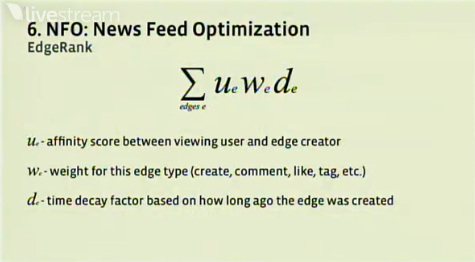
\includegraphics[width=0.5\columnwidth]{related/edgerankform2} 
\caption[News Feed Optimization formula]{NFO was designed to reduce the overload of information in Facebook NewsFeed. The algorithm took three parameters: affinity, time and weight. More information are available at \url{http://www.whatisedgerank.com/}. Source: \cite{f_EdgeRank3}}
\label{fig:nfo}
\end{figure}

%%%%%%%%%%
\section{Twitter engagement}
\paragraph{}
For a long time, Facebook has optimised its News Feed to spare its users from being overwhelmed by the vast amount of content that they receive. Research on Twitter is slightly different because the content is public and relatively controlled, seeing as a tweet is a message of less than 140 characters. The user can attach a photo, a video and hashtag. Thanks to this study \cite{t_fuel}, we have a better understanding of what facilitates engagement on twitter. The formula used to measure the rate is giving below Figure \ref{fig:t-engagement}.

\begin{figure}[h] 
\centering 
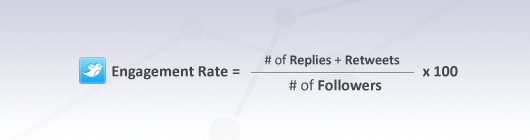
\includegraphics[width=0.6\columnwidth]{related/t-engagement} 
\caption[Twitter engagement rate]{The engagement rate is depending on the platform and the functionalities available. It is not an easy metrics to measure and has not a single formula. Find more information about it source \cite{f_t_engag_rates}}
\label{fig:t-engagement}
\end{figure}

This study shows that people do not engage equally with every Tweet. Indeed, adding extra content to the 140 limited characters increases considerably the engagement of the users. The Figure \ref{fig:t-retweets}, illustrates the fact that photos, videos and links are influential factors in increasing the number of retweets. \\
After considering the content of the tweets and the fact that images are increasing the number of retweets, we will discuss the design change that Twitter adopted in April 2014.

\begin{figure}[h] 
\centering 
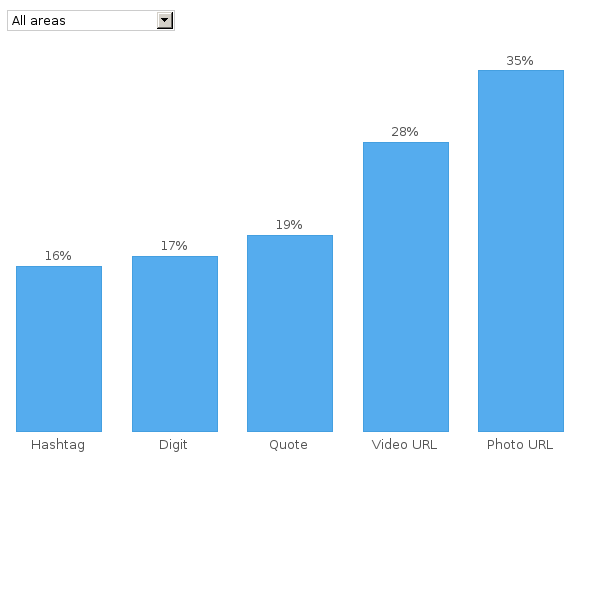
\includegraphics[width=0.7\columnwidth]{related/retweets} 
\caption[Level of retweet]{Engagement of people depending on the content added to the tweets, got from this source \cite{t_fuel}}
\label{fig:t-retweets}
\end{figure}


%%%%%%%%%%
\section{Twitter redesign}
\paragraph{}
In April 2014, Twitter launched its new design, instilling confidence in their investors. This modification, as shown in figure \ref{fig:twitter-new}, is modeled directly after the Facebook design.
With this adjustment, Twitter aimed to cut off the overload of information \cite{t_new_timeline}, taking the user back to the center of the platform. As with Facebook, users can now enjoy a larger profile photo, customize their header, and show off his best Tweets. 

\begin{figure}[h]
\centering 
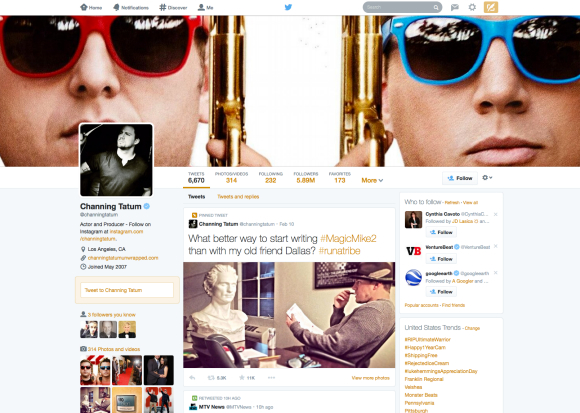
\includegraphics[width=0.8\columnwidth]{related/twitter-new} 
\caption[Twitter new design]{New design of a Twitter page. The profile picture and the Timeline remembers the Facebook design. The user is the central element of the page. Source: \cite{t_new_vs_old}}
\label{fig:twitter-new}
\end{figure}

Moreover, Twitter has developed some features to improve the content of the News Feed as it is mentioned on its blog \cite{t_new_design}:

\begin{itemize}
  \item \textbf{Best Tweets}: Tweets that have received more engagement will appear slightly larger, so your best content is easy to find.
  \item \textbf{Pinned Tweet}: Pin one of your Tweets to the top of your page, so it's easy for your followers to see what you're all about.
  \item \textbf{Filtered Tweets}: Now you can choose which timeline to view when checking out other profiles.
\end{itemize}

\paragraph{}
Engagement is a big issue for Social media companies, though its unclear definition makes it difficult to measure. We will try here to measure the difference between interest and engagement time and then find a way to increase the time spent on the Twitter news feed. In the next chapter, we will talk about the reasons why we chose this topic and how we reached it.